\documentclass[11pt,oneside,letterpaper]{article}

% graphicx package, useful for including eps and pdf graphics
\usepackage{graphicx}
\DeclareGraphicsExtensions{.pdf,.png,.jpg}

% basic packages
\usepackage{color} 
\usepackage{parskip}
\usepackage{float}

% text layout
\usepackage{geometry}
\geometry{textwidth=15cm} % 15.25cm for single-space, 16.25cm for double-space
\geometry{textheight=22cm} % 22cm for single-space, 22.5cm for double-space

% helps to keep figures from being orphaned on a page by themselves
\renewcommand{\topfraction}{0.85}
\renewcommand{\textfraction}{0.1}

% bold the 'Figure #' in the caption and separate it with a period
% Captions will be left justified
\usepackage[labelfont=bf,labelsep=period,font=small]{caption}

% review layout with double-spacing
%\usepackage{setspace} 
%\doublespacing
%\captionsetup{labelfont=bf,labelsep=period,font=doublespacing}

% cite package, to clean up citations in the main text. Do not remove.
\usepackage{cite}
%\renewcommand\citeleft{(}
%\renewcommand\citeright{)}
%\renewcommand\citeform[1]{\textsl{#1}}

% Remove brackets from numbering in list of References
\renewcommand\refname{\large References}
\makeatletter
\renewcommand{\@biblabel}[1]{\quad#1.}
\makeatother

\usepackage{authblk}
\renewcommand\Authands{ \& }
\renewcommand\Authfont{\normalsize \bf}
\renewcommand\Affilfont{\small \normalfont}
\makeatletter
\renewcommand\AB@affilsepx{, \protect\Affilfont}
\makeatother

% notation
\usepackage{amsmath}
\usepackage{amssymb}
\newcommand{\virus}{\mathbf{x}}						% virus coordinate
\newcommand{\serum}{\mathbf{y}}						% serum coordinate
\newcommand{\viruses}{\mathbf{X}}					% set of virus coordinates
\newcommand{\sera}{\mathbf{Y}}						% set of serum coordinates
\newcommand{\ve}{v}									% virus avidity
\newcommand{\se}{s}									% serum potency
\newcommand{\ves}{\mathbf{v}}						% set of virus avidities
\newcommand{\ses}{\mathbf{s}}						% set of serum potencies
\newcommand{\point}{f_{\scriptscriptstyle \vert}}	% point likelihood
\newcommand{\threshold}{f_{\textstyle \lrcorner}}	% threshold likelihood
\newcommand{\interval}{f_{\sqcup}}					% interval likelihood
\newcommand{\mdssd}{\varphi}						% MDS standard deviation
\newcommand{\virussd}{\sigma_x}						% virus / diffusion standard deviation
\newcommand{\serumsd}{\sigma_y}						% serum standard deviation
\newcommand{\drift}{\beta}							% drift / advection
\newcommand{\tree}{\tau}							% phylogeny
\newcommand{\vn}{n}									% number of viruses
\newcommand{\sn}{k}									% number of sera
\newcommand{\normal}{\mathcal{N}}					% normal distribution
\newcommand{\bwithin}{\beta_w}		% within clade drift coefficient
\newcommand{\bsister}{\beta_s}		% sister clade drift coefficient
\newcommand{\bother}{\beta_t}			% across clade drift coefficient
\newcommand{\incclade}[1]{y_\mathrm{#1}}
\newcommand{\driftclade}[1]{x_\mathrm{#1}}
\setlength{\arraycolsep}{2pt}
\newcommand{\smalltwomatrix}[2]{\scriptsize \Big( \begin{matrix} #1 \\ #2 \end{matrix} \Big)}				% pretty inline matrix 
\newcommand{\smallfourmatrix}[4]{\scriptsize \Big( \begin{matrix} #1 & #2 \\ #3 & #4 \end{matrix} \Big)}	% pretty inline matrix 
\newcommand{\twomatrix}[2]{\left( \begin{matrix} #1 \\ #2 \end{matrix} \right)}								% pretty inline matrix 
\newcommand{\fourmatrix}[4]{\left( \begin{matrix} #1 & #2 \\ #3 & #4 \end{matrix} \right)}					% pretty inline matrix 

%%% TITLE %%%
\title{\vspace{1.0cm} \Large \bf 
Clustering viruses using Antigenic Data and Phylogeny
}

\author[1]{Charles Y K Cheung}
\author[1]{Trevor Bedford}
\affil[1]{Vaccine and Infectious Disease Division, Fred Hutchinson Cancer Research Center, Seattle, WA}

\date{}

\begin{document}

\maketitle

%%% ABSTRACT %%%
\begin{abstract}

[to-do]
\end{abstract}

%%% IMPACT %%%
% Combined evolutionary and antigenic analysis shows that human influenza viruses differ dramatically in rates of antigenic drift and these rates significantly impact seasonal incidence patterns.

\pagebreak

%%% INTRODUCTION %%%
\section*{Introduction}

[How we write it really depends on the focus of the paper!]



If it's a method paper:

1. Something about this field
	- WHO
	- vaccine
	- HI assay


2. Antigenic Cartography
	- Derek's Smith's work
	- Trevor's .. capture uncertainty (why important?)
	- last sentence: but we want a tool to classify viruses

3. Scientific motivation for classifying viruses using HI titers.
	- and reasons to have a statistical method

4. What I precisely want to model, and why is there a missing gap

5. What I accomplished...



Some notes:

Trevor said, "WHO thinks about clusters... they don't think about what? [forgot what he said]...
"Fujian.. Beijing 92"
each phenotype's lifespan?
Antigenic variation...

"How much support do we have for a new virus?"



Main Motivations for Clustering

	- Classify viruses
	- Antigenically distinct subtypes
	- Correct antigenic location due to errors and uncertainties in measurements…
	- Detect driver mutations.. (later)

	- Want a model that explicitly makes use of the results from phylogenetic inference (tree)
	- Uses titer and information from sequence (through phylogenetic tree)
	- Believe single antigenic location per cluster
	- Simpler way of ensuring mixing - borrowing structure from phylogenetic inference
	- Want to know the relationship between clusters..
		○ Explicitly
	- Autocorrelation model
	- Want years…
	- Flexible number of clusters as determined by the algorithm
	
	- In the end we succeeded in capturing the essential features that we want to capture to focus on doing well in those things… and handling the technical aspect to improve MCMC mixing

Existing tool:
	- ddCRP
		○ Mixing..
		○ More simple model
		○ The speed of convergence
		○ Seeing misclassification…



\newpage

%%% MATERIALS AND METHODS %%%
\section*{Methods}

\subsection*{Overview}

We developed a method that simultaneously partitions viruses into antigenically distinct clusters and infers the locations of viruses on the antigenic map. 
Our work extends the original method for Antigenic Cartography (ref) and the Bayesian Multidimensional Scaling Dimension approach (ref) to summarize information from the HI data in lower dimension to succintly represent the overall relationship between viruses and sera.
In this work, we further leverage an inferred phylogenetic tree, which provides valuable information about the evolution process of viruses, to infer distinct antigenic clusters of viruses and their locations in the antigenic map.


\subsection*{Posterior inference}


\begin{equation}
  p(Y, I, \mu ) \propto  p(H|Y, X(\mu, I, T) ) p(Y| t ) p(I) p(\mu)
\end{equation}

Our model has several components.
The term $p(H|Y, X(\mu, I, T) )$ specifies the antigenic likelihood of the observed titer measurements $H$.
In this antigenic likelihood, $H$ is explained by the locations of sera $Y = (Y_1, ..., Y_{n_{s}} )$ and viruses $X=(X_1, ..., X_{n_v} )$ in a two-dimension antigenic map.
Whereas $Y$ is controlled by the prior $p(Y|t)$ that depends on the date of serum $t$,
 $X$ is determined by the phylogenetic tree $T$ and parameters $\mu$ and $I$.
$I$ and $\mu$ are specified by the prior $p(I)$ and $p(\mu)$, respectively.

[note potential confusion between $t$ and $T$]


\subsection*{Autocorrelation Model for Virus Locations and the Prior for Serum Locations}

First, we partition viruses into distinct antigenic clusters using a previously inferred $T$ (Figure~\ref{autocorrelationModel}).
$T$ is composed of N total nodes that includes external nodes representing the set of viruses and internal nodes connecting the external nodes.
Each node $i$ has a binary indicator variable $I_i$ that is active if $I_i=1$ or inactive if $I_i=0$. 
If $I_i=1$, node $i$ and all its descending nodes are branched off into a new cluster from the parent of node $i$.
Thus, we can assign all viruses into distinct clusters by traversing $T$ using $I = (I_1, ... I_N)$.



%%% Illustration of the autocorrelation model %%%
\begin{figure}[h]
	\centering		
	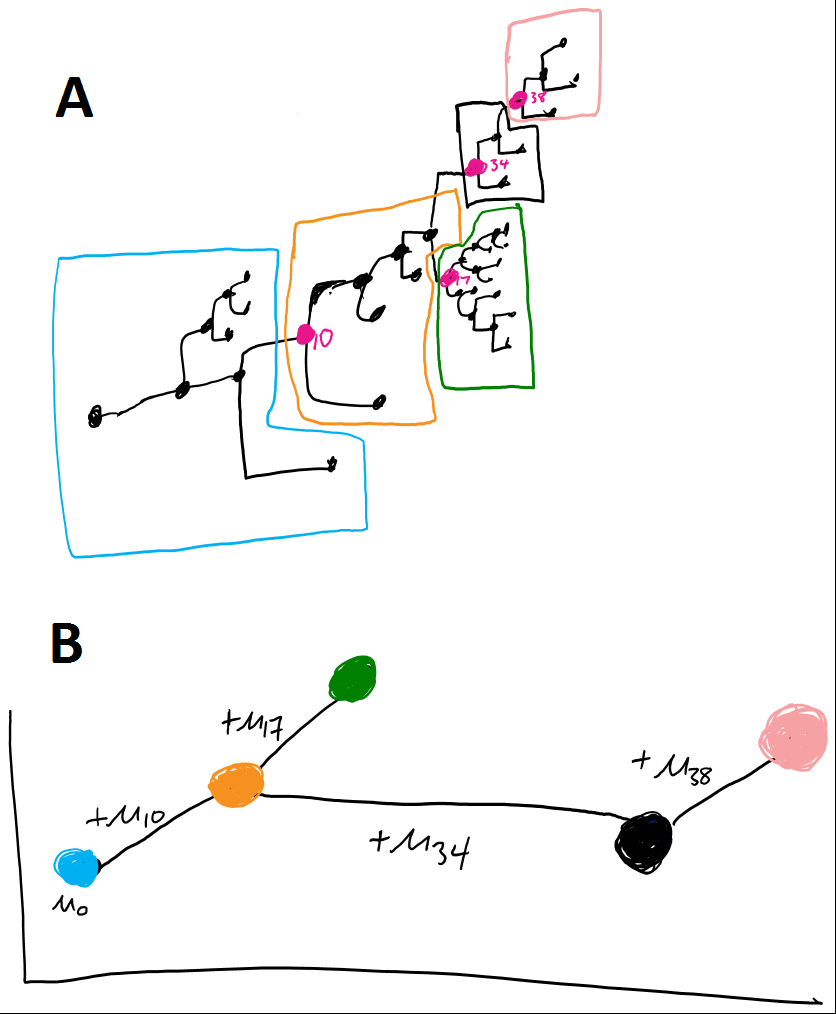
\includegraphics[width=0.5\textwidth]{figures/autocorrelationModel}
	\caption{\textbf{Phylogenetic Clustering and Autocorrelation model.} 
(A) Each node on this phylogenetic tree $T$ is represented by a circle. 
Node 10, 17, 34, and 38 are active (purple; $I_{10}=I_{17}=I_{34}=I_{38}=1$) and each remaining node is inactive (black; $I_i=0$). 
These active nodes partition the viruses, which are the external nodes, into 5 clusters.
(B) Antigenic map of viruses are drawn using the set of $\mu_i$s that are associated with the $T$ and $I$ above. 
For example, the green and black clusters are branched off from the orange cluster. 
The blue cluster is the root cluster that is given an initial location $\mu_1$  \textbf{[need to think how to parametrize!]}.
	} 
	\label{autocorrelationModel} 
\end{figure}

[Note: the $\mu_0$ ... $\mu_k$, and root cluster being turned on by default? issue]

Second, we assign antigenic locations to viruses ($X$). 
Our model assumes that all viruses in the same cluster share the same antigenic coordinate and viruses in different clusters have different antigenic coordinates.
This modeling decision is motivated by the evidence that a small fraction of driver mutations contribute to substantial antigenic drift while most of them do not(Koel), so our priority here is to parsimoniously model the most substantial antigenic changes.
The use of autocorrelation parametrization is inspired by the Relaxed Molecular Clock model where ... (cite).


We are ultimately only interested in the location of the $n_v$ viruses $X=(X_1,..., X_{n_{v}})$, but to determine their values, we need to work with an augmented space $X' = (X_1, ...X_{n_v}, X_{ n_v +1},..., X_N)$ that consists of the locations of not only the external (viruses) but also the internal $(X_{ n_{v}+1}, ... X_N)$ nodes.
Initially, we define
\begin{eqnarray}
 	X_{k} = \mu_k  
\end{eqnarray}
, where $k$ is the index of the root node and $\mu_k$ is a parameter to be estimated. 
Second, we traverse the entire set of nodes in $T$ in a top-down fashion from the root node to assign antigenic locations of the remaining nodes by using the autocorrelation model
\begin{equation}
	X_i=  X_{p(i)} + \mu_i    I_i   
\end{equation}
, for each of $i=1,... N$, where $p(i)$ is a function that returns the index of the parent of node $i$.
Thus, if $I_i=0$, node i has identical location as that of its parent, and if $I_i=1$, the location of node i is different than its parent by $\mu_i$.
At the end of the tree traversal, $X'$, and thus X, will have been deterministically assigned [given the current value of $I$ and $\mu$].




Our use of indicator variables is commonly referred to be the Bayesian Stochastic Search Variable Selection procedure (cite). Here, each indicator $I_i$, for $i=1,..N$, follows the prior

\begin{equation}
 p(I_i = 1) = p
\end{equation}
, where $p$ is a \textbf{user-specified value} between 0 and 1, with small value penalizing a node from branching off into a new cluster.


We assume an independent and identically distributed normal prior for $\mu_i$, $i=1,...N$, where $\sigma^2_u$ is \textbf{an user-specified value} and $I$ is the identity matrix with 1 in the diagonal and 0 in the off-diagnoal cells. [Note. need another symbol. I is used.]

\begin{equation}
   \mu_i  \sim N_2 ( (0,0)' , \sigma^2_u I) 
\end{equation}


This autocorrelation model has a few desirable properties.
First, this model partitions viruses in a very natural way that is related to the evolution process as specified by $T$.
It allows us to understand the path in which clusters transition.
Second, the parametrization allows us to easily infer the change in antigenic distance from one cluster to the next.
Third, we keep this model simple and intuitive, so we can focus on the essential aspects that we want to capture.



For the antigenic locations of sera, we used the previously introduced Diffusion model  (paper). We assumed a normal prior on the antigenic location of sera.
\begin{eqnarray}
	y_i | t_i \sim N_2 ( m_0, \sigma^2_s I)  \\
	m_0 = ( \drift t_i ,0)' \nonumber
\end{eqnarray}
where $t$ is the difference between the date of the indexed virus or serum and the date of the earliest sampled virus or serum and $\sigma^2_s$ is \textbf{currently a fixed value}. 
With the mean of the first dimension scaled by the year offset of serum, this drift prior has an effect of spreading out the serum locations by years, a property which we think is reasonable because virus evolves over time (? good enough justification?). 
\textbf{For convenience, we currently set $\beta  = 1$ .}


\subsection*{Implementation}


We use the Markov-chain Monte Carlo technique (ref) to sample from the posterior distribution.
We have experimented with various Metropolis Hasting proposals to evaluate, understand, and optimize the mixing behavior. 
After that, we retained a small subset of proposals.
These proposals for $\mu$ and $I$ are classified into three types: essential, efficient, and situational. 

%%  Table of proposals we kept %%
\begin{table}[h]
	\centering
	\caption{\textbf{List of retained MCMC proposals for $\mu$ and $I$  } }
	\label{errortable}	
	\makebox[\textwidth][c]{
	\small
	\begin{tabular}{ c c c } 
	\hline
	
Type		& no.	& Proposal description\\
Essential	& 1	& Choose an $\mu_i$ randomly and propose from the prior\\
	& 2	& Choose an $I_i$ randomly and flip status and balance active $\mu$\\
\hline
Efficient	& 3	& Swap the status between a random active $I_i$ and an inactive $I_j$\\
	& 4	& Swap $I_i$ and $\mu_i$ with a neighbor\\
	& 5	& Walk an active $\mu_i$ and balance other active $\mu$\\
\hline
Situational 	& 6	&  Swap $I_i$ and $\mu_i$ with a hot neighbour\\
 	& 7	& Swap with a neighbor and Flip $I$ of another neighbor \\

	\hline
	\end{tabular}	
	}
\end{table}



We retained two essential proposals that theoretically ensures ergodicity of the chain toenable the chain to move through the entire space. 
In the first proposal (no.1), we randomly choose a $\mu_i$ to change, and $\mu_i$ is changed to a new value sampled independently from the prior distribution of $\mu_i$. 
We retained this proposal instead of an alternative proposal that performs a random walk from the existing value of $\mu_i$ because with the tree containing many nodes, the latter proposal would take much longer to draw representative samples.
In the second proposal (no.2), we randomly choose a binary $I_i$ to flip status and change some of the required $\mu$'s to balance the virus locations of neighboring clusters (Figure~\ref{flipAndBalance}). Precisely, 


\begin{equation}
\label{flipI-equation}
I_i^{new} = \left\{
\begin{array}{llll}
	   1 & & : & I_i^{existing} =  0 \\
	   0  & & : & otherwise
\end{array}
\right.
\end{equation}

is accompanied by 

\begin{equation}
\label{muBalance-equation}
	\mu_j^{new} =  \left \{
\begin{array}{lllr}
    \mu_j^{existing} - \delta		& &	: I_i^{new} = 1\\
    \mu_j^{existing} + \delta	& &	: otherwise
\end{array}
\right.
\end{equation},
for each index $j$ in which $I_j = 1 $  and forms a new children cluster from the cluster generated by node $i$. Balancing these active $\mu$'s minimizes the impact that flipping on or off $I_i$ has on the antigenic map, so the proposal would have a higher chance of acceptance. Trivially, this proposal allows all theoretical combinations of $I$, and proposals no.1 and 2, along with proposals for other parameters, are sufficient for exploring the entire space.



%%% Illustration of the flip and balance %%%
\begin{figure}[h]
	\centering		
	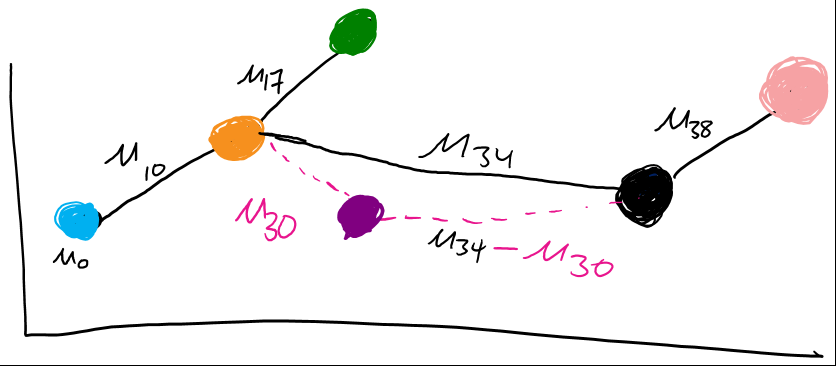
\includegraphics[width=0.5\textwidth]{figures/flipAndBalance}
	\caption{\textbf{Proposal 2 - Flip indicator and balance.} 
In this antigenic map, the purple cluster represents the new cluster of viruses generated by flipping $I_{30}$ from 0 to 1. In order to fix the absolute location of viruses in the black and pink clusters,  $\mu_34$ has to be adjusted by the value of $\mu_{30}$.
	} 
	\label{flipAndBalance} 
\end{figure}



We retained three (four) efficient proposals that are practically important for MCMC mixing. 
Proposal no.3 switches status between a randomly chosen active $I_i$ with another randomly chosen inactive $I_i$. 
This proposal gets accepted more often than proposal no.2 most likely because the prior of $I_i$ penalizes for an increase in the number of active nodes in no.2.

Proposal no.4 swaps both the $I$ and $\mu$ in a pair of nodes, but instead of swapping a random pair, the pivot active node is swapped with a node that is within a user-defined neighborhood from it as defined by $T$ (Figure~\ref{multistep}) (and excluding the pivot node).
Within the neighborhood with $n_{c}$ candidates , the proposal randomly picks from this set of possibilities with equal probability $\frac{1}{n_{c}}$.
This proposal has two desirable properties:
First, swapping $I$ with a neighbor is much more efficient than swapping $I$ between two arbitrarily far nodes (as in no.3) because the former proposal makes a much smaller change to the virus partitioning than the latter proposal.
Second, by also swapping $\mu$, the new active neighbour gets the value of $\mu_i$ from the now inactive pivot, so the virus assignment but not the cluster locations change. 
We learned that swapping $\mu$ allows higher observed acceptance rate ($3.2\%$) than not swapping $\mu$ ($1.1\%$), so we decided to includes swapping $\mu$ in proposal no.4.


%%% Illustration of the swap with neighbor proposal %%%
\begin{figure}[h]
	\centering		
	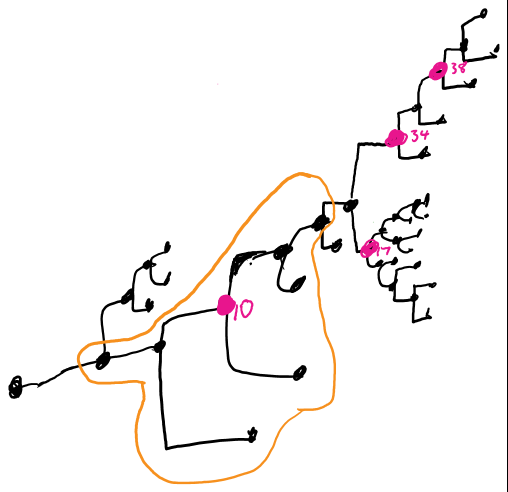
\includegraphics[width=0.5\textwidth]{figures/multistep}
	\caption{\textbf{Proposal 4 - Swap $I_i$ and $\mu_i$ with a neighbor} 
In this $T$, node 10 is chosen to perform the swap with neighbor proposal. With a neighborhood step-size of 2, the set of candidates are all the nodes within the orange neighborhood minus node 10.
	} 
	\label{multistep} 
\end{figure}



Proposal no.5 selects a random dimension of a random active $\mu_i$ whose $I_i = 1$ to change while keeping the absolute location of other clusters fixed (Figure~\ref{walkAndBalance}). Precisely, 
\begin{equation}
	\mu_i^{new} =  \mu_i^{existing} + \delta \\
\end{equation},
where $\delta \sim \frac{1}{2} (U(-M, M), 0)' + \frac{1}{2} (0, U(-M, M))'$ and $M$ is the walk size specified by the user.
Similar to that in proposal no.2, the balancing move of other clusters is accomplished by
\begin{equation}
	\mu_j^{new} =  \mu_j^{existing} - \delta\\
\label{balance_mu}
\end{equation},
for each index $j$ in which $I_j = 1 $  and forms a new children cluster from the cluster generated by node $i$. 



%%% Illustration of the walk an active mu and balance proposal%%%
\begin{figure}[h]
	\centering		
	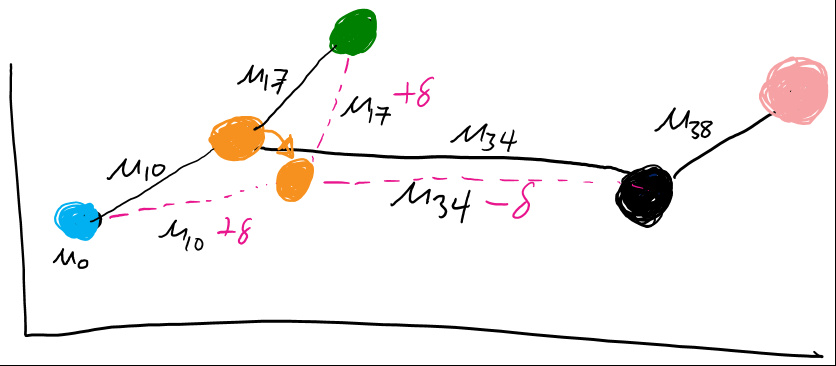
\includegraphics[width=0.5\textwidth]{figures/walkAndBalance}
	\caption{\textbf{Proposal 5 - Performs a random walk on an active $\mu_i$ and balance other $\mu$'s.} 
In this antigenic map, $\mu_{10}$ is now changed by $\delta$, which causes the antigenic location of viruses in the orange cluster to change. 
To retain the absolute location of viruses in other clusters,  $\mu_{17}$ and $\mu_{34}$ are adjusted by subtracting $\delta$.
	} 
	\label{walkAndBalance} 
\end{figure}


There are three reasons why we included this proposal.
First, in contrast to proposal no.1, here the proposal only focuses on the active $\mu$s, which are the $\mu$'s that influence the antigenic likelihood.
Second, in contrast to proposal no.1., this proposal performs a random walk because if $\mu$ is from an active node, we learned from profiling the proposal that the random walk operator has dramatically higher chance of acceptance (16.4$\%$) than sampling from independent prior proposal ($0.x\%$), largely because an active $mu$ tends to have high likelihood in a preferred region of the space.
Third, by balancing the active $\mu$'s of the children clusters, we increase the chance of acceptance ( equation \ref{flipI_equation} + \ref{muBalance-equation} = 26.1$\%$ vs. equation \ref{flipI_equation} only =16.4$\%$).



We also included two proposals that we referred to as "situational" because they may not be necessary but may situationally help with MCMC mixing.
The first proposal (no.6) is a companion of proposal no. 4. 
In a separate routine, we first record the frequency of which the MCMC chain accepts a change in $I$ and updates this list in every user-defined (e.g. 100,000) number of steps from all other proposals.
The set of nodes that are called accepted are called the "hot" nodes. 
Proposal no.6 is identical to proposal no.4 except that only the "hot" nodes can be candidates to swap to. 
By limiting the number of nodes to consider, this proposal has shown to be accepted up to 4 times more than proposal no. 4 when $p$ is set to be very small (p=0.001?), likely because in this situation a new indicator does not get accepted very often?? (think more why!)
[For simplicity, we decided not to use this proposal unless p is small, because under the default $p=0.02$, the improvement was not too substantial.]
The second booster proposal (no.7) combines proposal no. 4 with flipping the indicator of a neighbor node. 
Precisely, in the flip step, the proposal searches for the union of the set of neighbors from the existing node and the set of neighbors from the new node and each of the node in this union set has an equal chance to be selected (Figure~\ref{jointMultistep}).
The second proposal may potentially help a cluster to branch off into two clusters and vice versa.

%%% Illustration of the swap with a neighbor and flip another neighbor proposal%%%
\begin{figure}[h]
	\centering		
	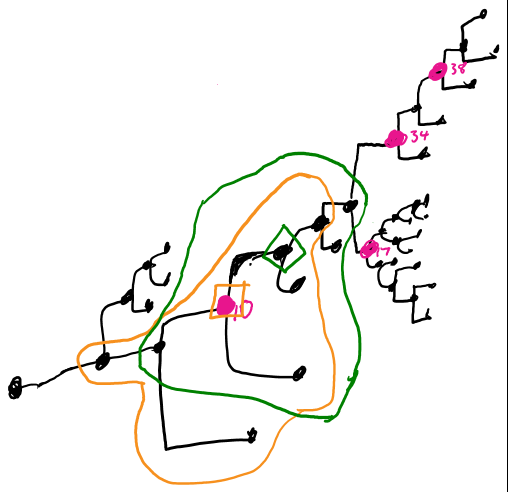
\includegraphics[width=0.5\textwidth]{figures/jointMultistep}
	\caption{\textbf{ The candidate of nodes to be flipped in Proposal 7 - Swap with a neighbor and flip another neighbor.} 
In the second operation that flips the indicator status of another neighbor, the list of nodes to consider include neighbors from the original pivot node and the neighbors of the newly chosen node. 
Taking the union of the two set of nodes allows a node that may be further away to be chosen and also ensures that the Metropolis-Hasting ratio would be greater than 0 because the backward operation from the new state to the old state would also have a probability greater than 0.
	} 
	\label{jointMultistep} 
\end{figure}

  [perhaps further explain the motivating example: the 604 $<-->$ 605, 592 situation]




For other parameters, we inherited proposals from the previous work (ref). We used a random walk operator that is similar to that in equation \ref{muBalance-equation} to explore the space each $Y_i$. 


\newpage




\subsection*{Antigenic Likelihood }

[Need to paraphrase]


\begin{equation}
 p(H|Y, X(\mu, I, T)) = \prod_{(i,j) \in \cal I} f(H_{ij} | Y_i, X_i (\mu, I, T)) 
\end{equation}



\begin{equation}
	\delta_{ij} =  || \virus_i - \serum_j ||_2,
\end{equation}
where $|| \cdot ||_2$ is an $L_2$ norm.



\begin{equation}
	d_{ij} =  \se_j - H_{ij},
\end{equation}
where $H_{ij}$ is the log$_2$ titer of virus $i$ against serum $j$ and serum potency $\se_j = \max ( H_{1j},\ldots,H_{\vn j} )$ is fixed.
In following multidimensional scaling, these approaches attempt to optimize over unknown $\viruses$ and $\sera$ such that
\begin{equation} \label{mds}
	\sum_{(i,j) \in \cal I} 
	\left(
		\delta_{ij} - d_{ij}
	\right)^2
\end{equation}
is minimized, where $\mathcal{I} = \{ (i,j) : H_{ij} \mbox{ is measured} \}$.



\begin{equation} \label{hij}
	H_{ij} \sim \normal( \se_j - \delta_{ij}, \, \mdssd^2 ).
\end{equation}
Consequently, the likelihood of observing an exact titer given the placement of antigenic locations is 
\begin{equation} 
	\point(H_{ij}) = \phi \left( \frac{ H_{ij} + \delta_{ij} - \se_j }{ \mdssd } \right),
\end{equation}
where $\phi(\cdot)$ represents the standard normal probability density function (PDF).



\begin{equation} 
	\threshold(H_{ij}) = \Phi \left( \frac{ H_{ij} + \delta_{ij} - \se_j }{ \mdssd } \right),
\end{equation}
where $\Phi(\cdot)$ represents the standard normal cumulative distribution function (CDF).




\begin{equation} 
	\interval(H_{ij}) = \Phi \left( \frac{ H_{ij} + \delta_{ij} - \se_j + 1 }{ \mdssd } \right) - \Phi \left( \frac{ H_{ij} + \delta_{ij} - \se_j }{\mdssd} \right).
\end{equation}


\subsection*{Analysis using Hemagluttination Inhibitation Assay Data and Phylogeny}

Trevor's...
Collected H3N2 data from ....
spanning 39 years


402 viruses, 
5xx sera


MCC tree from TreeAnnotator version 1.x?, 803? nodes



Run conditions:

Default setting: full dataset, $p$ = 0.02, $\sigma^2_\mu$ = 4 ,   $\sigma^2_s$ = ?, $mds-precision$ = 0.01, 

number of clusters depends on the vaule of a few parameters, so I try a few...

\newpage

%%% RESULTS %%%
\section*{Results and discussion}





%%% Result Figure %%%
\begin{figure}[h]
	\centering		
	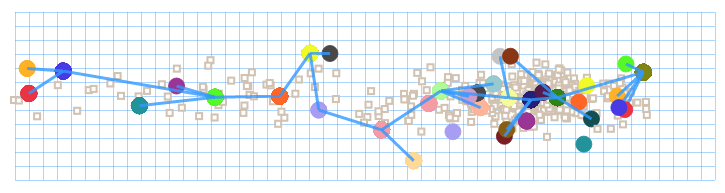
\includegraphics[width=1\textwidth]{figures/fullData-MCC-Euclid-50M}
	\caption{\textbf{Full dataset} 
[to write]
	} 
	\label{MyLabel} 
\end{figure}


%%% Result Figure %%%
\begin{figure}[h]
	\centering		
	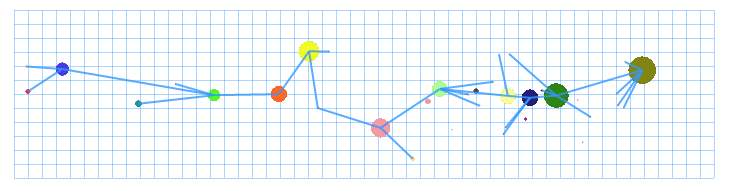
\includegraphics[width=1\textwidth]{figures/fullData-MCC-Euclid-50M-proportional}
	\caption{\textbf{Full dataset} 
[to write]
	} 
	\label{MyLabel} 
\end{figure}

%%% Result Figure %%%
\begin{figure}[h]
	\centering		
	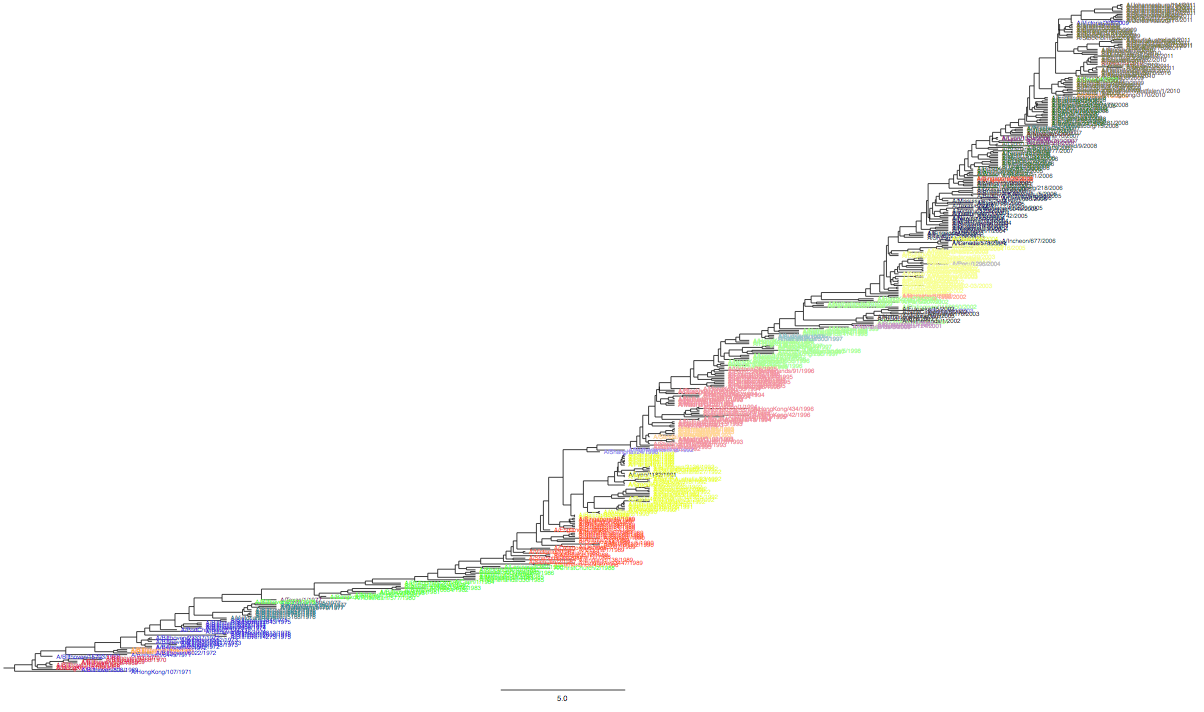
\includegraphics[width=0.8\textwidth]{figures/fullData-MCC-figTree-50M}
	\caption{\textbf{Full dataset} 
[to write]
	} 
	\label{MyLabel} 
\end{figure}


\newpage

%%% Result Figure %%%
\begin{figure}[h]
	\centering		
	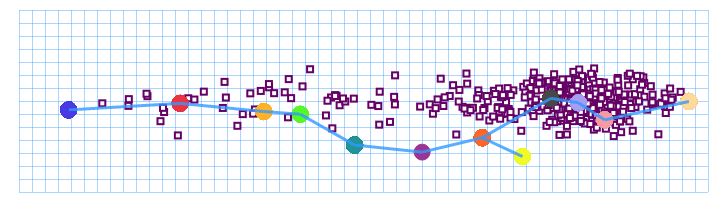
\includegraphics[width=0.8\textwidth]{figures/thinnedData-MCC-Euclid-50M}
	\caption{\textbf{Thinned dataset} 
[to write]
	} 
	\label{MyLabel} 
\end{figure}

%%% Result Figure %%%
\begin{figure}[h]
	\centering		
	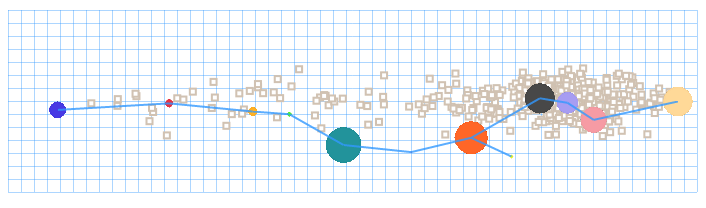
\includegraphics[width=0.8\textwidth]{figures/thinnedData-MCC-Euclid-50M-proportional}
	\caption{\textbf{Thinned dataset} 
[to write]
	} 
	\label{MyLabel} 
\end{figure}

%%% Result Figure %%%
\begin{figure}[h]
	\centering		
	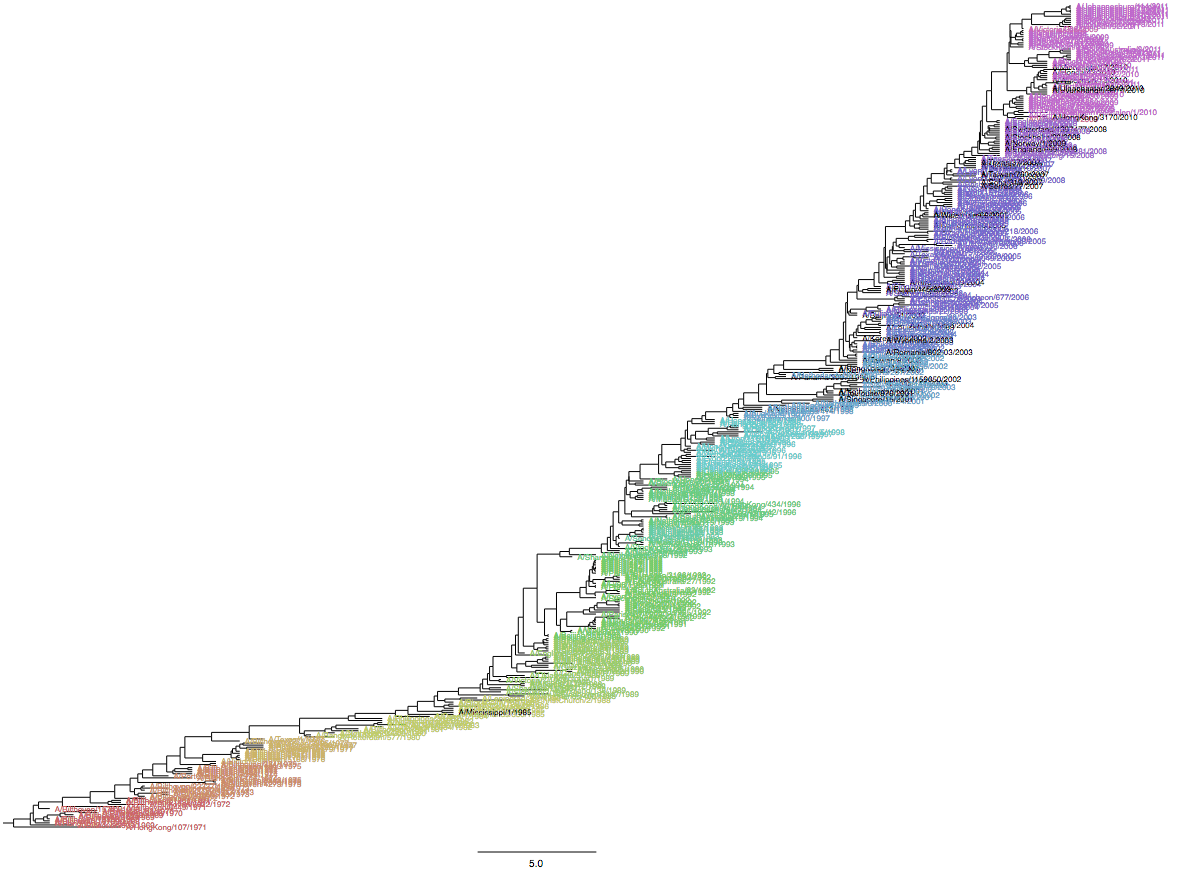
\includegraphics[width=0.72\textwidth]{figures/thinnedData-MCC-figTree-50M}
	\caption{\textbf{Thinned dataset} 
[to write]
	} 
	\label{MyLabel} 
\end{figure}


\newpage

[todo]


Clustering

Euclid results

antigenic distances





Potential Discussion items:
  - also, pulled along the viruses in a natural way which makes it easy for the MCMC to go through that space...
  - maybe a discussion item: - We tried the version without... not as effective in placing the viruses in the correct spot... spiral thing.....)


philosophy is to have the algorithm simple to understand and also focus on technical stuff..


\newpage












\newpage


[maybe, or maybe no need: Please refer to the appendix for more information regarding various other proposals.
We kept a few of those moves from the original set.]

 decisions..
[done]     - propose from independent prior  - instead of walking
[done]     - multistep on as an efficient move for exchanging...
[done]	     - multistep has to balance.. (much more efficient than not)
     - flipI
	-needed, also has to balance
	- not very popular because the prior... but that's the way it is

     - the onMultistepExchange Mu and Flip Another I
	- but there, we need to "walk"
    - "hot multistep" vs. multistep
	    - but usually turned off here because it doesn't add much in some settings.

    - the Y and mu joint moves and other stuff don't seem to necessarily help much. (low acceptance rate... get rid to increase overall efficiency )
    - "on" move...



Furthermore, we have proposals 

\iffalse
number	Proposal	Acceptance Rate
0	Proposal_changeToAnotherNodeOn	0.008782835371967114
1	Proposal_changeMuFromPrior	0.9829411529703168
2	Proposal_flipIandChangeMu	0.0036237719439523274
3	Proposal_changeAnOnMuWalk	0.16383817260516367
4	Proposal_multistepOnNode	0.010833973400169786
5	Propose_YandMu	0.014037192561487702
6	Propose_YandI	0.007877496885173425
7	Propose_YandIandmu	0.007842659189727336
8	Propose_branchOffFlip	0.003125761143135504
9	Propose_multistepOnNodeFlipMu	0.03211896510034658
10	Propose_flipI	0.0036910732196589768
11	Propose_changeOnMuAndBalance	0.2606520335700452
12	Proposal_changeMuFromWalk	0.7980458656330749
14	Propose_HotMultistepOnNodeFlipMu	0.055140862027450034
15	Proposal_flipIBalance	0.004056224899598394
16	Proposal_OnMultistepIExchangeMuAndFlipAnotherI	0.007367526211391329
17	Proposal_changeRootMuWalk	0.049723756906077346
18	Proposal_changeRootMuWalkAndBalance
\fi







\subsection*{From Trevor}


Let $\virus_i \in \mathbb{R}^{P}$ represent the cartographic location of virus $i$ for $i = 1,\ldots,\vn$, so that $\virus_i = (x_{i1}, x_{i2})^{\prime}$ for $P=2$. 
Similarly, let $\serum_j$ represent the cartographic location of serum $j$ for $j = 1,\ldots,\sn$, so that $\serum_j = (y_{j1},y_{j2})^{\prime}$ for $P=2$.
For notational compactness, we collect together all virus coordinates into an $\vn \times P$ matrix  $\viruses = (\virus_1, \ldots, \virus_{\vn})^{\prime}$ and all serum coordinates into an $\sn \times P$ matrix $\sera = (\serum_{1},\ldots,\serum_{\sn})^{\prime}$.
Virus and serum may be isolated from / raised against the same strain and have different cartographic locations, and separate serum isolates raised against the same strain may also have different cartographic locations. 
This gives a set of distances between virus and serum cartographic locations 
\begin{equation}
	\delta_{ij} =  || \virus_i - \serum_j ||_2,
\end{equation}
where $|| \cdot ||_2$ is an $L_2$ norm.

Traditional approaches to antigenic cartography \cite{Smith04} begin by defining immunological distance as
\begin{equation}
	d_{ij} =  \se_j - H_{ij},
\end{equation}
where $H_{ij}$ is the log$_2$ titer of virus $i$ against serum $j$ and serum potency $\se_j = \max ( H_{1j},\ldots,H_{\vn j} )$ is fixed.
In following multidimensional scaling, these approaches attempt to optimize over unknown $\viruses$ and $\sera$ such that
\begin{equation} \label{mds}
	\sum_{(i,j) \in \cal I} 
	\left(
		\delta_{ij} - d_{ij}
	\right)^2
\end{equation}
is minimized, where $\mathcal{I} = \{ (i,j) : H_{ij} \mbox{ is measured} \}$.
In the case of threshold measurements, this error function is modified slightly; see \cite{Smith04} for further details.

Here, we instead assume a probabilistic interpretation in which an observed titer is normally distributed around its cartographic expectation with variance $\mdssd^2$,
\begin{equation} \label{hij}
	H_{ij} \sim \normal( \se_j - \delta_{ij}, \, \mdssd^2 ).
\end{equation}
Consequently, the likelihood of observing an exact titer given the placement of antigenic locations is 
\begin{equation} 
	\point(H_{ij}) = \phi \left( \frac{ H_{ij} + \delta_{ij} - \se_j }{ \mdssd } \right),
\end{equation}
where $\phi(\cdot)$ represents the standard normal probability density function (PDF).
Previous BMDS has employed a sampling density truncated to strictly positive quantities since $d_{ij}$ are directly observed, non-negative quantities.  
In the antigenic setting, these remain random and can be negative since neither $\se_j$ is known nor is $H_{ij}$ observed with much precision. 

HI assays sometimes show no inhibition at all measured titrations, e.g.\ a measurement can be reported as `$<$40'.
In this case, the likelihood of observing the threshold measurement follows the cumulative density of the lower tail of the normal distribution
\begin{equation} 
	\threshold(H_{ij}) = \Phi \left( \frac{ H_{ij} + \delta_{ij} - \se_j }{ \mdssd } \right),
\end{equation}
where $\Phi(\cdot)$ represents the standard normal cumulative distribution function (CDF).


\begin{equation} 
	\interval(H_{ij}) = \Phi \left( \frac{ H_{ij} + \delta_{ij} - \se_j + 1 }{ \mdssd } \right) - \Phi \left( \frac{ H_{ij} + \delta_{ij} - \se_j }{\mdssd} \right).
\end{equation}


We calculate the overall likelihood by multiplying probabilities of individual measurements
\begin{equation}  \label{bmds}
	L(\viruses,\sera) = \prod_{(i,j) \in \cal I} f(H_{ij}),
\end{equation}
using probability functions $\point$, $\threshold$ and $\interval$ as appropriate.

%%% REFERENCES %%%
\bibliographystyle{plos}
\bibliography{antigenic_clustering}

\end{document}
